\documentclass[letterpaper,12pt]{report}
\usepackage[pdftex]{graphicx}
\usepackage[spanish]{babel}
\usepackage[latin1]{inputenc}
\pagestyle{plain}

\begin{document}
\addtolength{\textwidth}{-3cm}
\begin{figure}
\chapter{UML}

%%%%%%%%%%%%%%%%%%%%%%%%%% CLASE  C45 %%%%%%%%%%%%%%%%%%%%%%%%%%%%%%%%%%%%%%%%%%%%

\section{Clase C45}
\centering
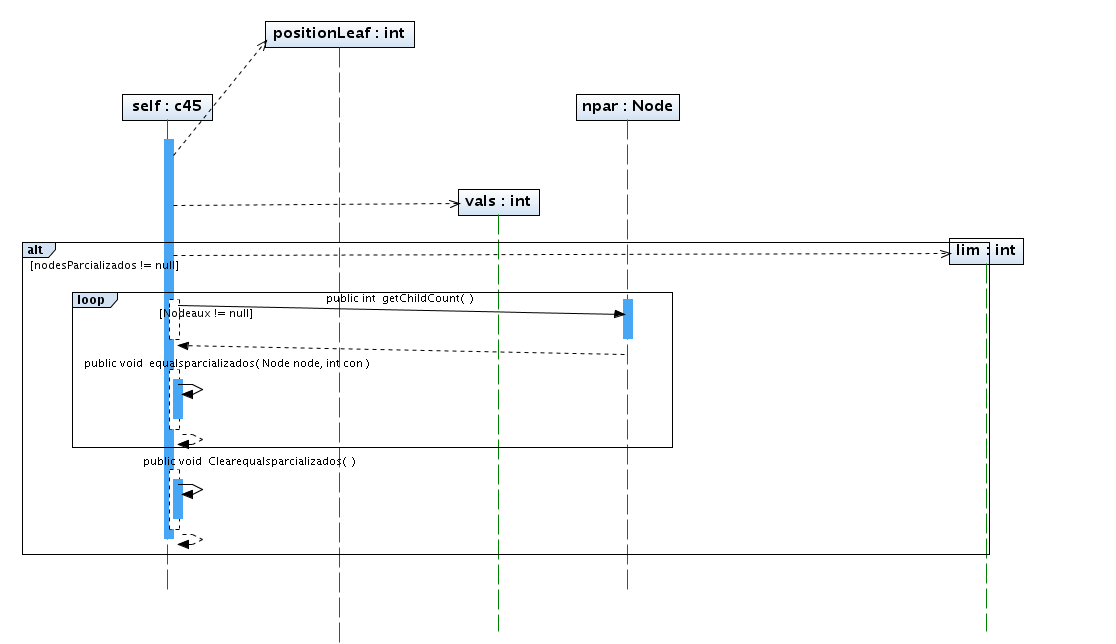
\includegraphics[width=1.2\textwidth]{c45/C45Clearequalsparcializados.png}
\caption{C45Clearequalsparcializados}
\end{figure}
\newpage
\begin{figure}
\centering
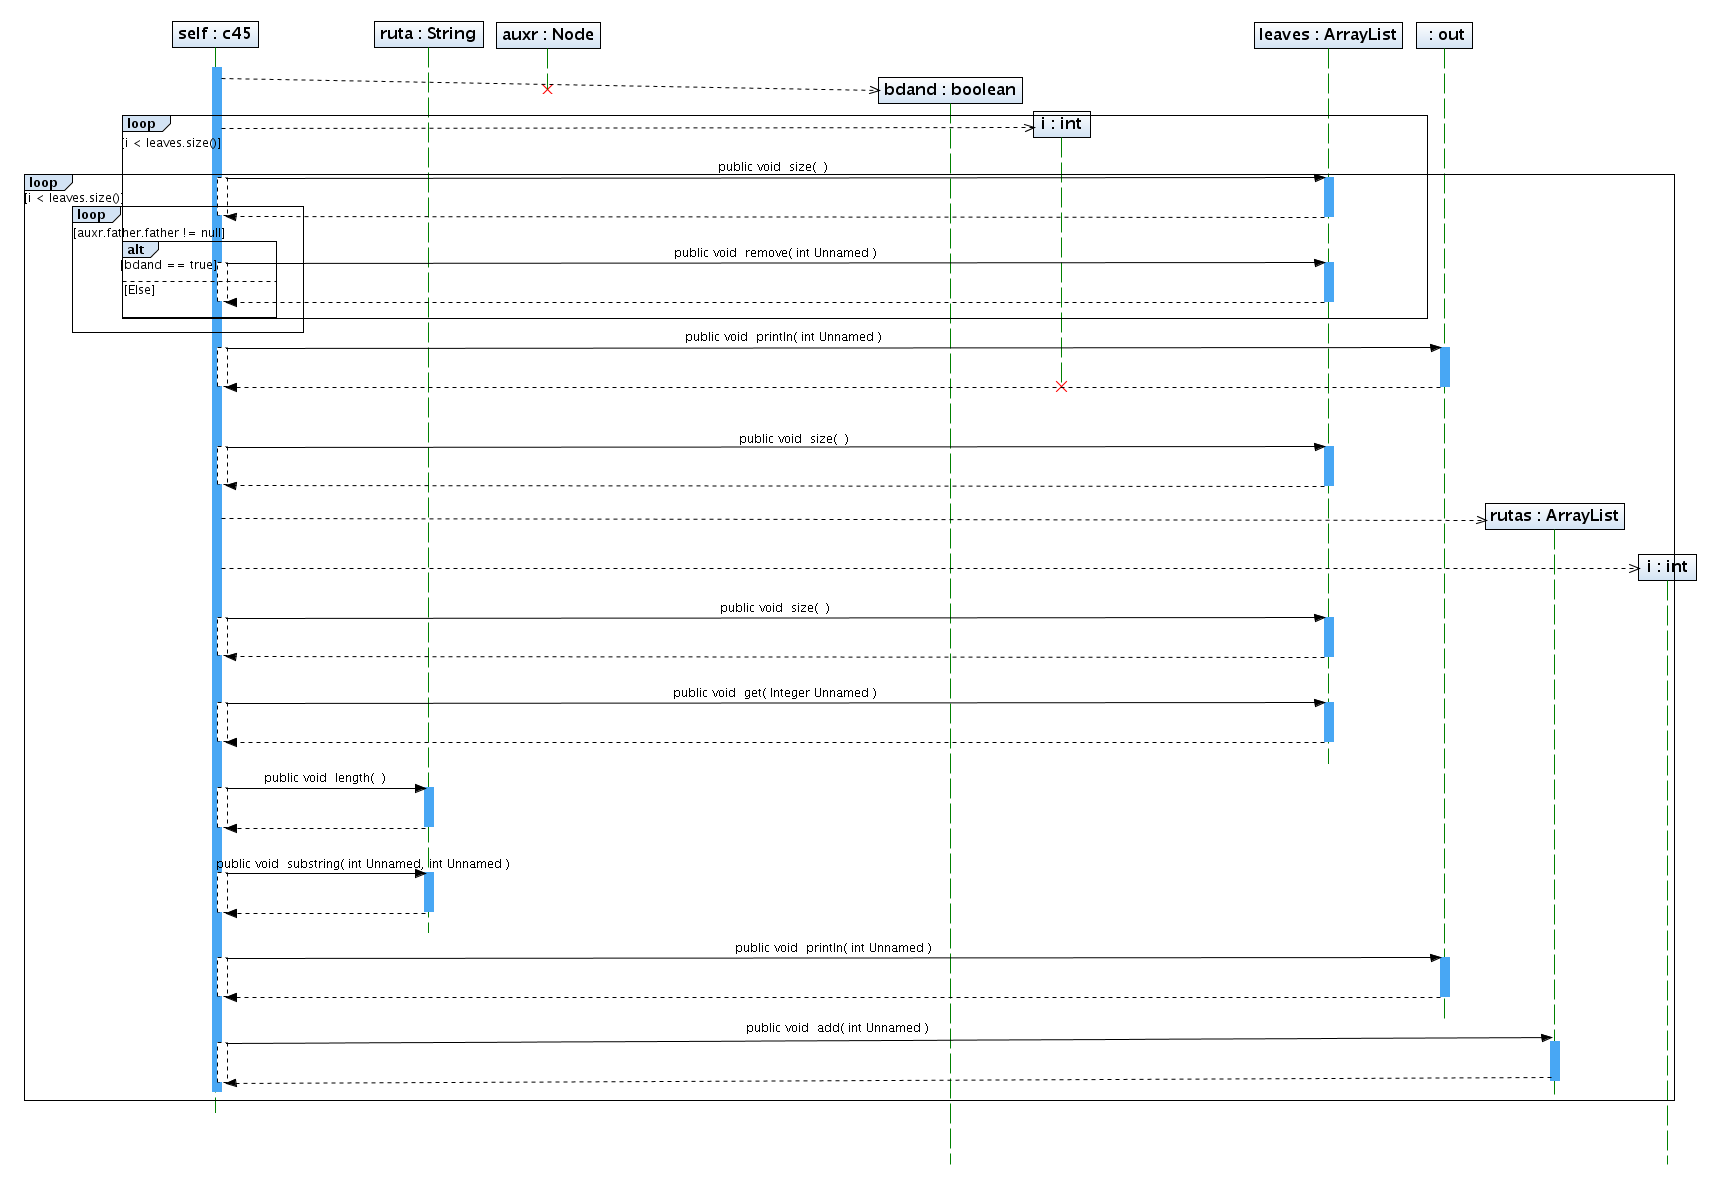
\includegraphics[angle=90, width=1\textwidth]{c45/C45Rules.png}
\caption{C45Rules}
\end{figure}
\newpage


%%%%%%%%%%%%%%%%%%%%%%%%%% CLASE  myHasMap %%%%%%%%%%%%%%%%%%%%%%%%%%%%%%%%%%%%%%%%%%%%
\begin{figure}
\section{Clase myHasMap}
\centering
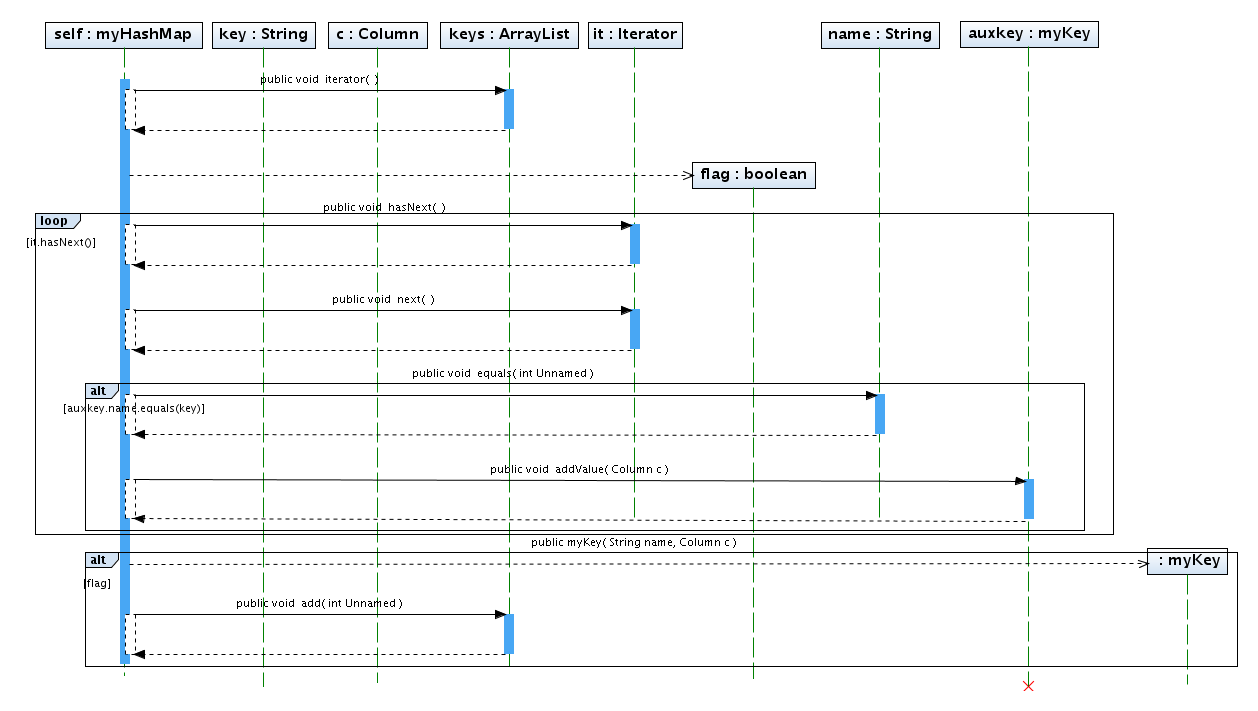
\includegraphics[angle=90, width=0.8\textwidth]{myHasMap/addColumn.png}
\caption{addColumn}
\end{figure}
\newpage
\begin{figure}
\centering
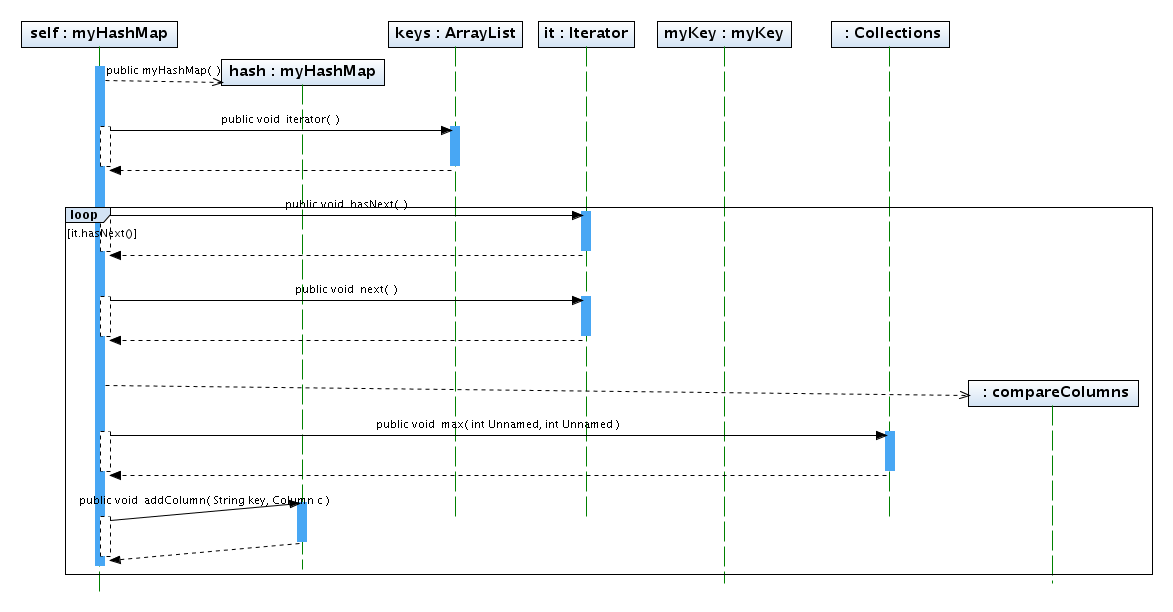
\includegraphics[angle=90, width=0.8\textwidth]{myHasMap/SearchColumn.png}
\caption{SearchColumn}
\end{figure}
\newpage


%%%%%%%%%%%%%%%%%%%%%%%%%% CLASE  Route %%%%%%%%%%%%%%%%%%%%%%%%%%%%%%%%%%%%%%%%%%%%

\begin{figure}
\section{Clase Route}
\centering
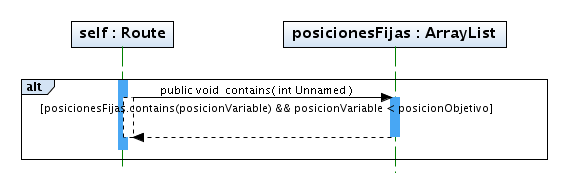
\includegraphics[width=1\textwidth]{Route/avanceVariable.png}
\caption{avanceVariable}
\end{figure}
\newpage
\begin{figure}
\centering
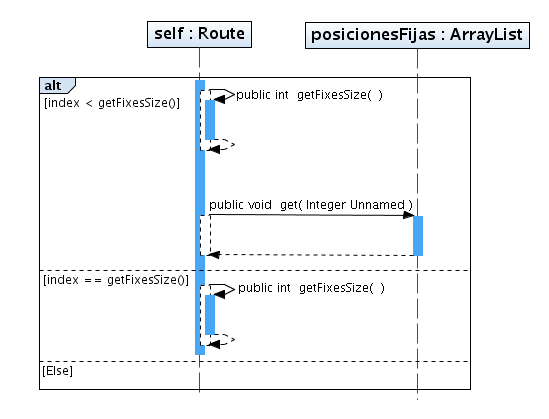
\includegraphics[width=1\textwidth]{Route/getIndex.png}
\caption{getIndex}
\end{figure}
\newpage
\begin{figure}
\centering
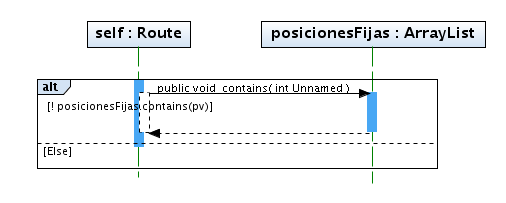
\includegraphics[width=1\textwidth]{Route/setPoscicionVariable.png}
\caption{setPoscicionVariable}
\end{figure}
\newpage

%%%%%%%%%%%%%%%%%%%%%%%%%% CLASE  TreeCounter %%%%%%%%%%%%%%%%%%%%%%%%%%%%%%%%%%%%%%%%%%%%

\begin{figure}
\section{Clase TreeCounter}
\centering
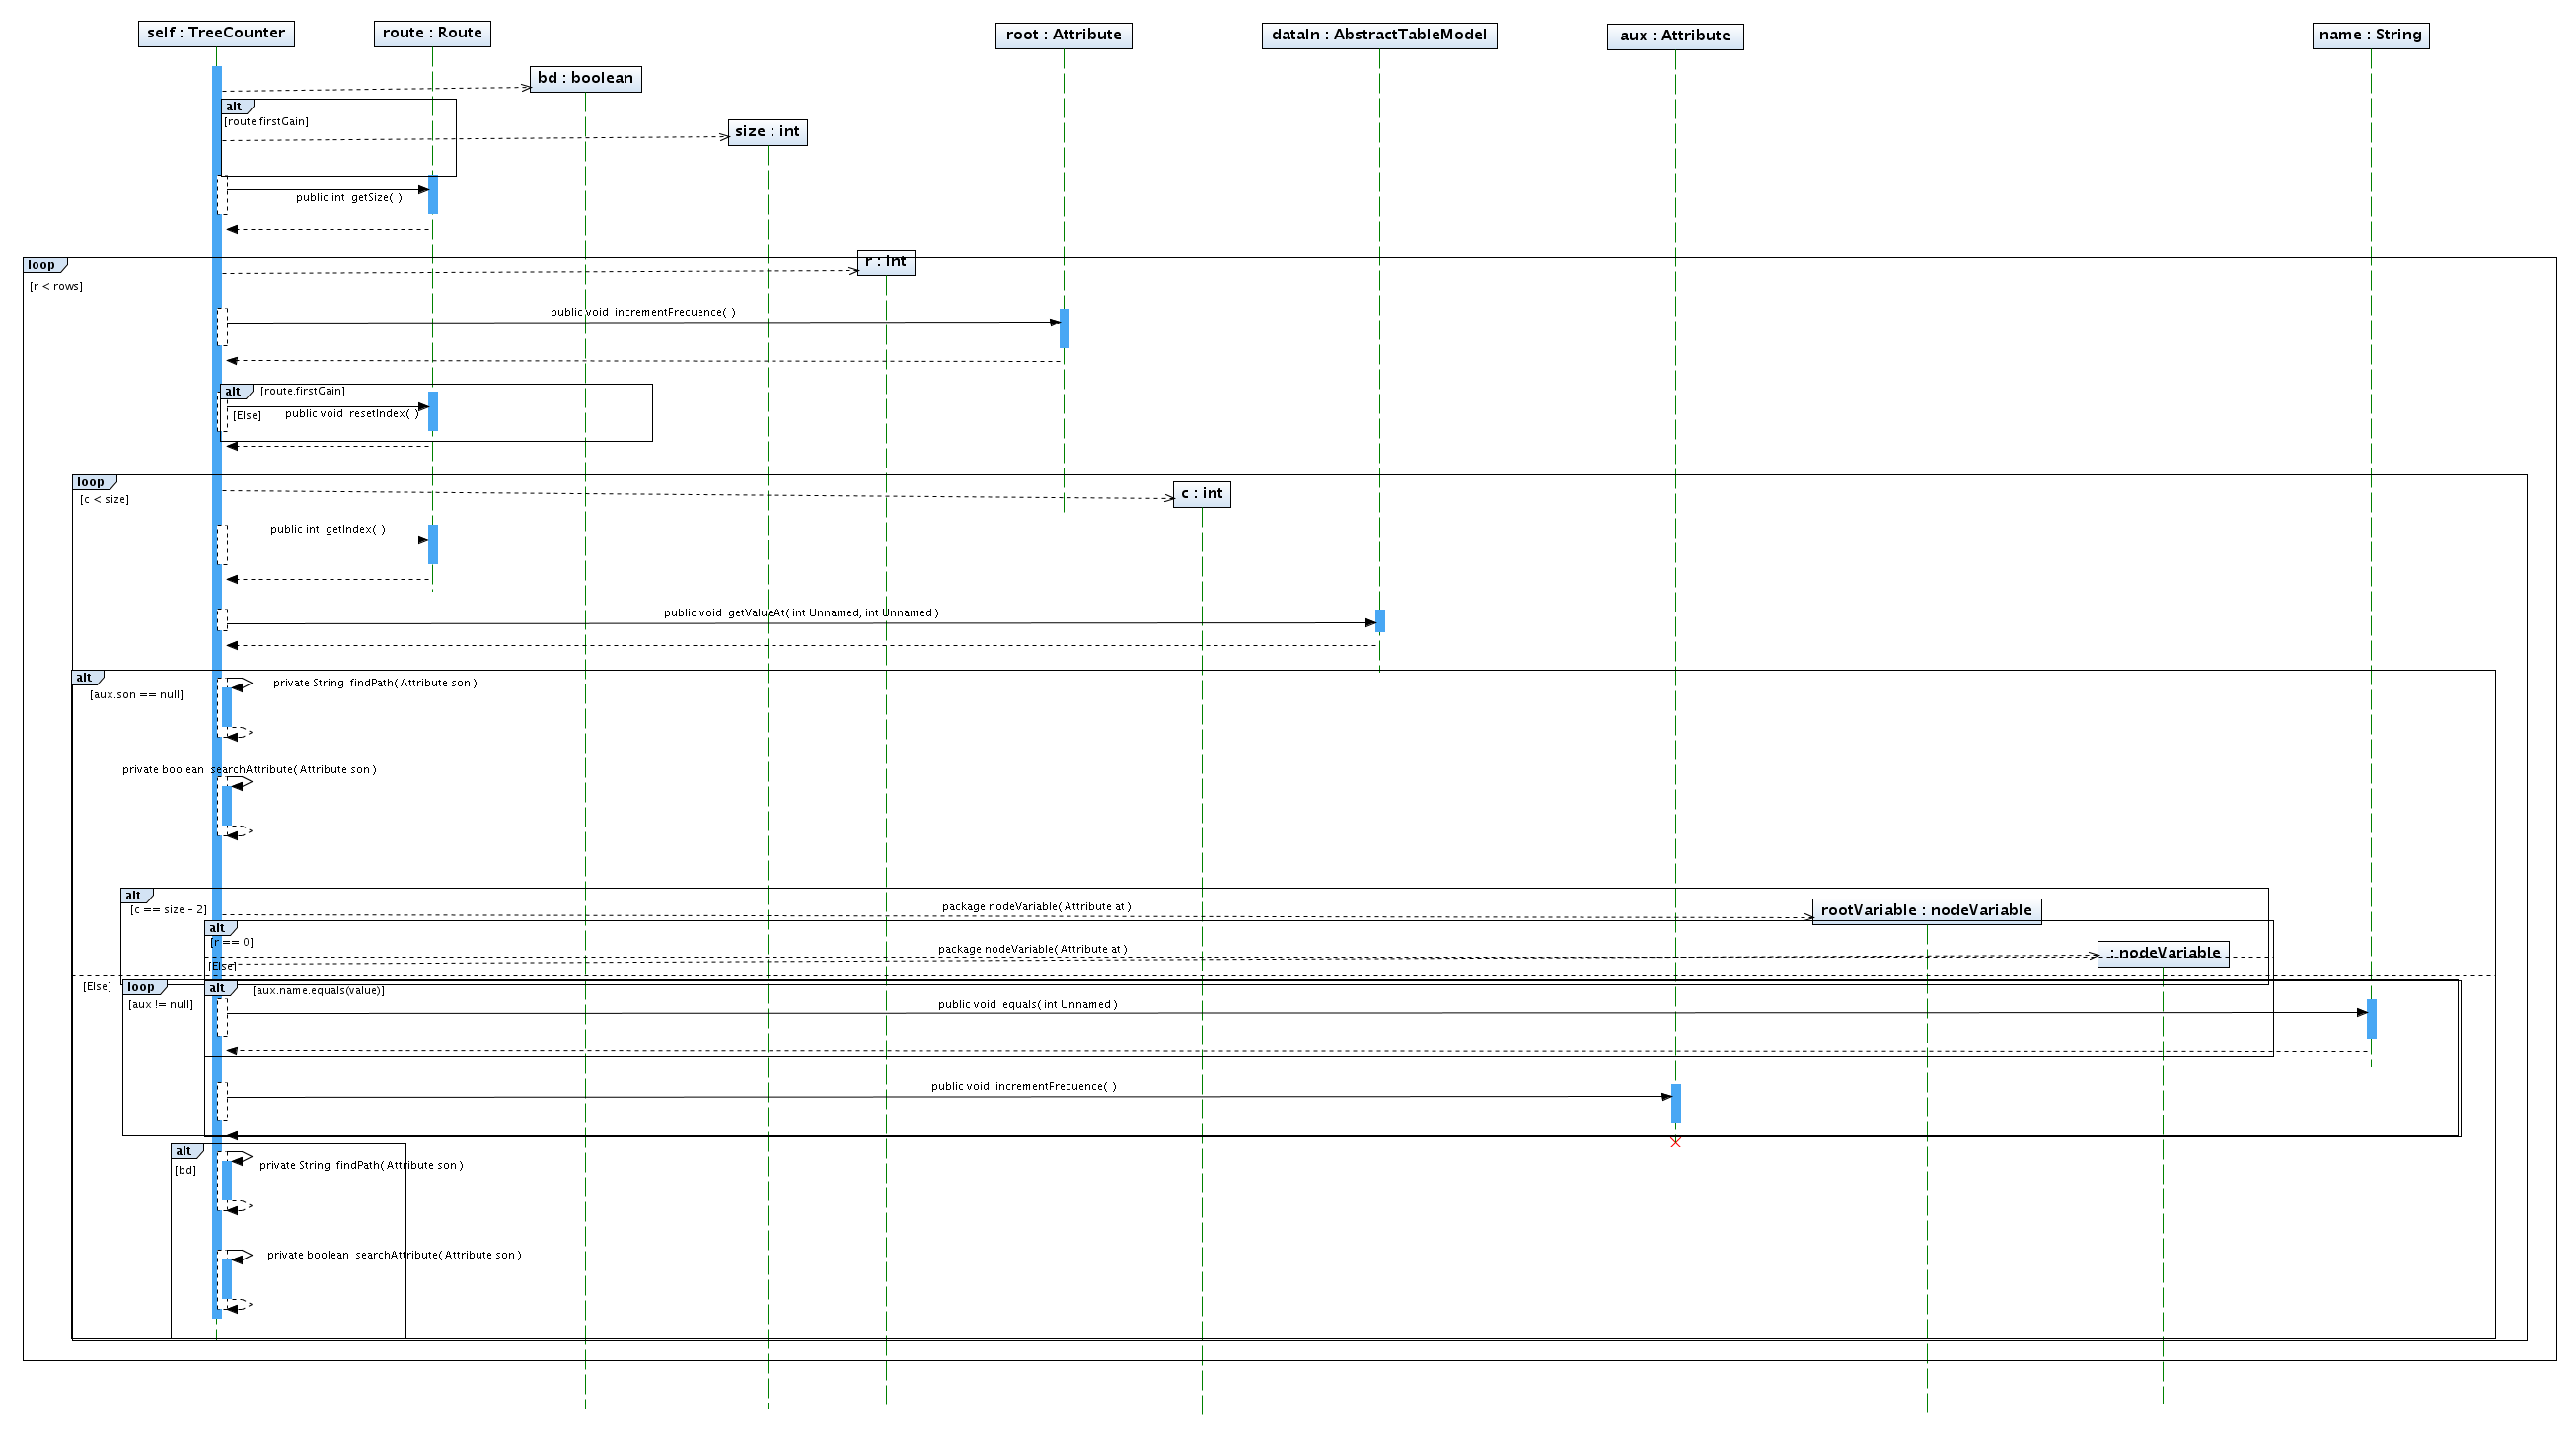
\includegraphics[angle=90, width=0.8\textwidth]{TreeCounter/createTree.png}
\caption{createTree}
\end{figure}
\newpage
\begin{figure}
\centering
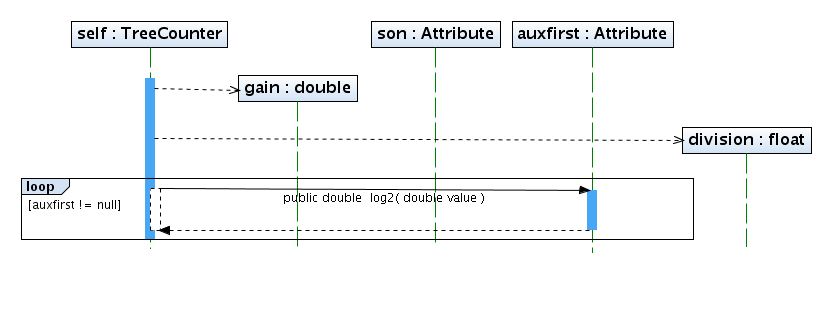
\includegraphics[width=1\textwidth]{TreeCounter/gananciaInicial.png}
\caption{firstGain}
\end{figure}
\newpage
\begin{figure}
\centering
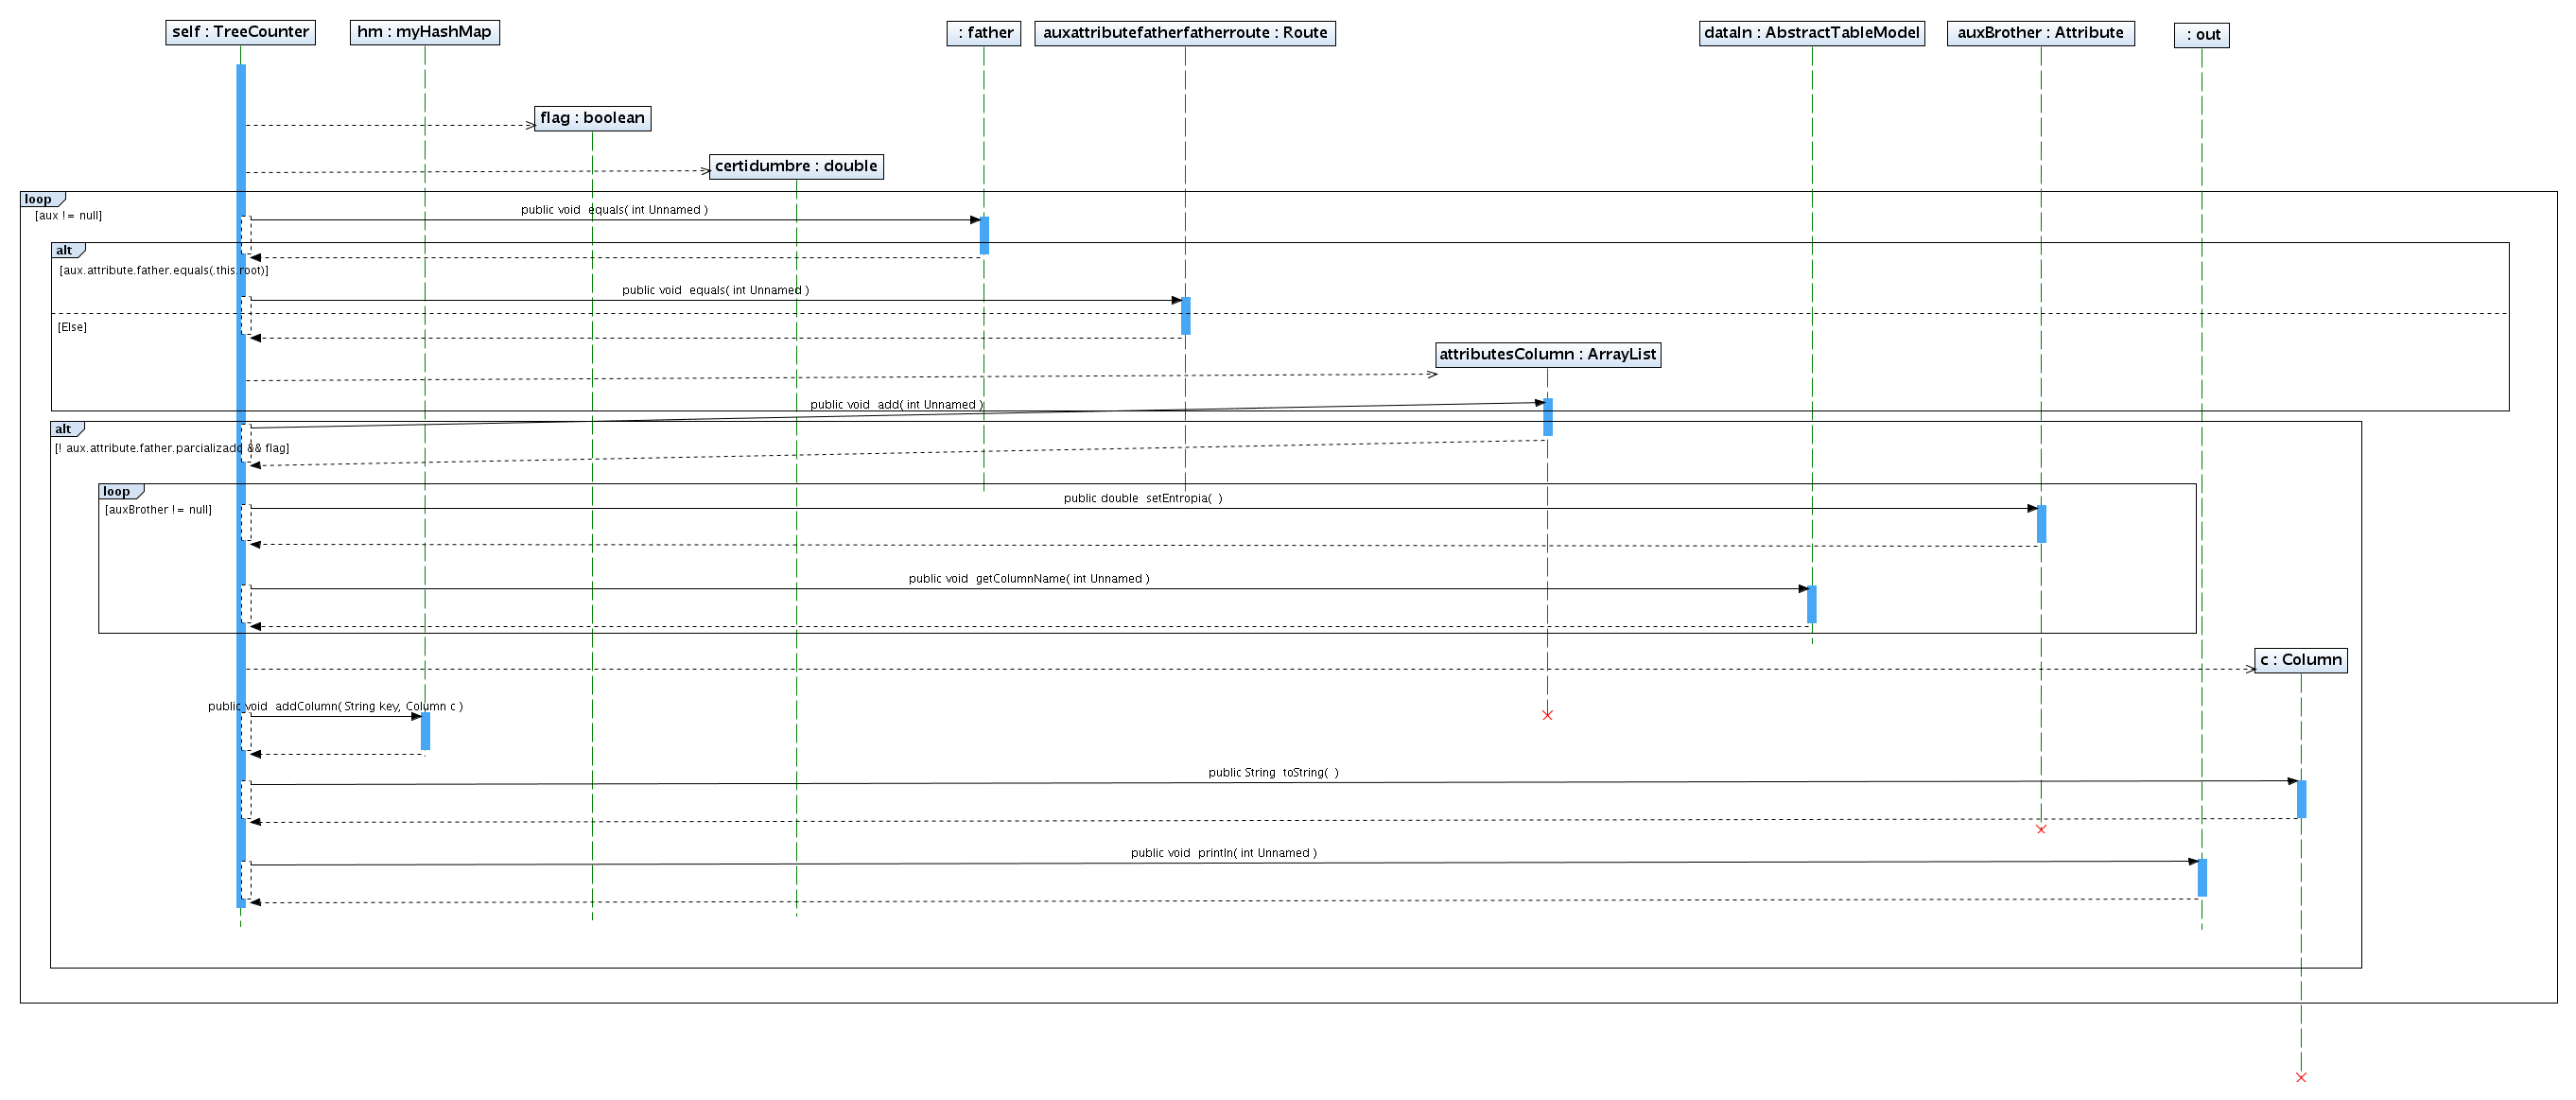
\includegraphics[angle=90, width=0.7\textwidth]{TreeCounter/ganancia.png}
\caption{gain}
\end{figure}
\newpage
\begin{figure}
\centering
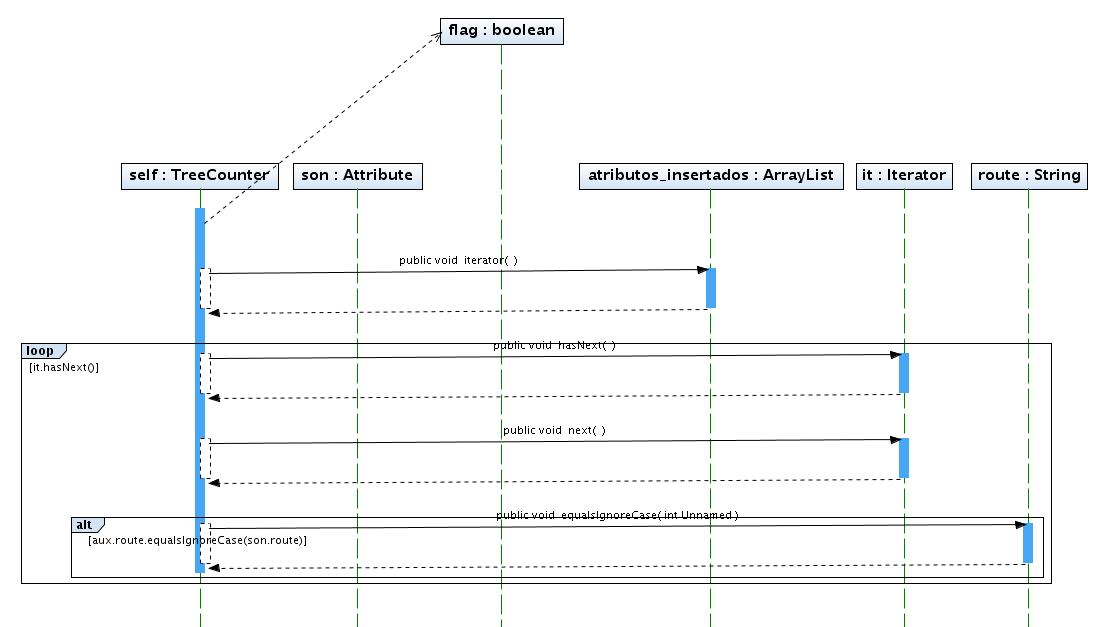
\includegraphics[width=1\textwidth]{TreeCounter/searchAttribute.png}
\caption{searchAttribute}
\end{figure}
\newpage
\begin{figure}
\centering
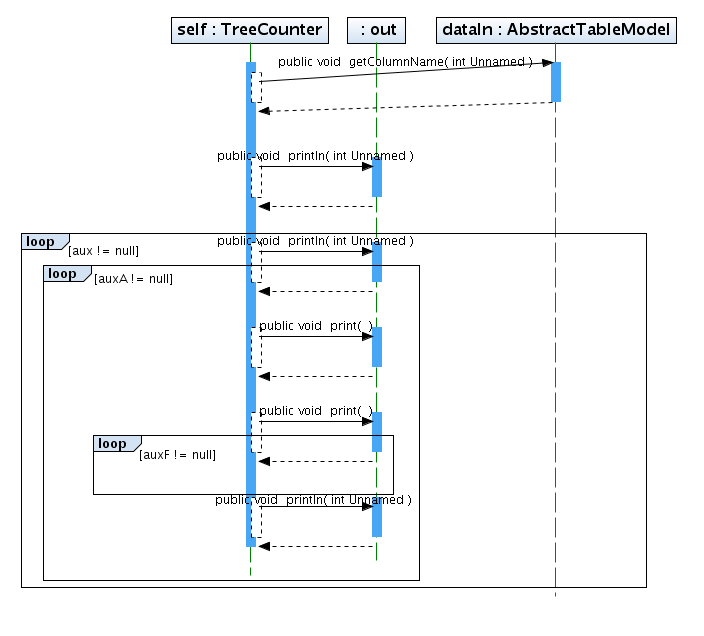
\includegraphics[width=1\textwidth]{TreeCounter/seeTree.png}
\caption{seeTree}
\end{figure}
\newpage

%%%%%%%%%%%%%%%%%%%%%%%%%% CLASE  Attribute %%%%%%%%%%%%%%%%%%%%%%%%%%%%%%%%%%%%%%%%%%%%

\begin{figure}
\section{Clase Attribute}
\centering
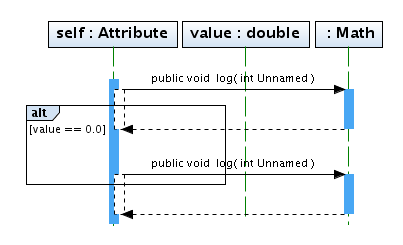
\includegraphics[width=1\textwidth]{Attribute/log2.png}
\caption{log2}
\end{figure}
\newpage
\begin{figure}
\centering
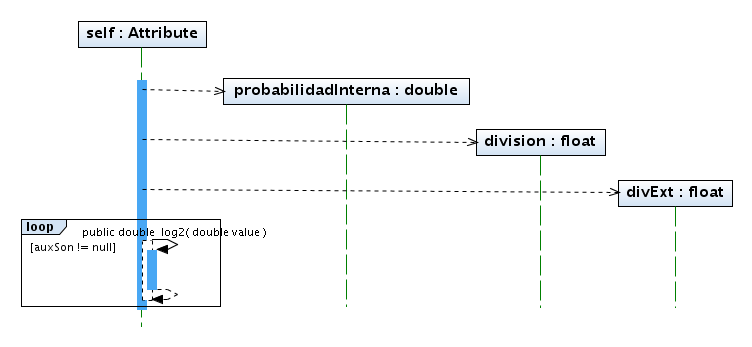
\includegraphics[width=1.2\textwidth]{Attribute/setEntropia.png}
\caption{setEntropia}
\end{figure}
\newpage


%%%%%%%%%%%%%%%%%%%%%%%%%% CLASE  Node %%%%%%%%%%%%%%%%%%%%%%%%%%%%%%%%%%%%%%%%%%%%

\begin{figure}
\section{Clase Node}
\centering
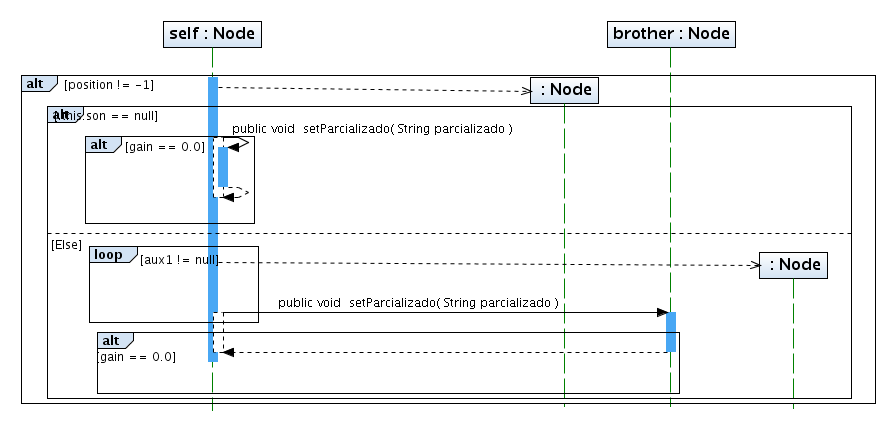
\includegraphics[width=1.2\textwidth]{Node/addSon.png}
\caption{addSon}
\end{figure}
\newpage
\begin{figure}
\centering
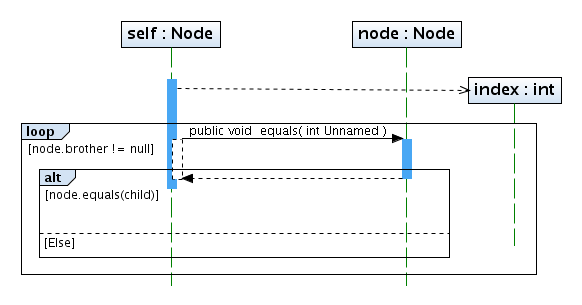
\includegraphics[width=1\textwidth]{Node/getIndexOfChild.png}
\caption{getIndexOfChild}
\end{figure}
\newpage

\end{document}
